% CoFuse4D MoSca-style method figure for Section 1.3.1.
% Figure-specific source images live in the adjacent assets/ directory.
\begingroup
\linespread{1}\selectfont
\definecolor{cfBlue}{HTML}{2E6DA4}
\definecolor{cfBlueBg}{HTML}{EAF3FB}
\definecolor{cfGreen}{HTML}{2E7D4F}
\definecolor{cfGreenBg}{HTML}{EAF6EE}
\definecolor{cfOrange}{HTML}{B9770E}
\definecolor{cfOrangeBg}{HTML}{FDF4E3}
\definecolor{cfRed}{HTML}{C0392B}
\definecolor{cfCyan}{HTML}{00A8C0}
\definecolor{cfGray}{HTML}{7F8C8D}
\definecolor{cfInk}{HTML}{1F2A36}
\begin{tikzpicture}[
  x=1cm,y=1cm,line cap=round,line join=round,text=cfInk,
  font=\songti\fontsize{8pt}{9.8pt}\selectfont,
  every node/.style={align=center,outer sep=0pt,inner sep=0pt},
  cfStage/.style={draw,line width=.9pt,dash pattern=on 4pt off 2.5pt,rounded corners=2.5pt},
  cfTitle/.style={font=\heiti\fontsize{9.2pt}{11pt}\selectfont},
  cfSub/.style={font=\heiti\fontsize{7.6pt}{9pt}\selectfont},
  cfSmall/.style={font=\songti\fontsize{7.2pt}{8.8pt}\selectfont},
  cfTiny/.style={font=\songti\fontsize{6.6pt}{8pt}\selectfont},
  cfArrow/.style={draw=cfGray,line width=2.2pt,-{Latex[length=3.0mm,width=2.4mm]}},
  cfThinArrow/.style={draw=cfInk,line width=.55pt,-{Latex[length=1.2mm,width=.8mm]}}
]
  \useasboundingbox (0,0.10) rectangle (14.75,9.02);

  % ================= (A) foundation =================
  \path[cfStage,draw=cfBlue,fill=cfBlueBg] (0.10,4.75) rectangle (4.35,8.90);
  \node[cfTitle,text=cfBlue,anchor=west] at (0.28,8.62) {(A) 基础观测};
  % input filmstrip
  \foreach \x/\f in {0.30/input_00000.png,1.45/input_00118.png,2.60/input_00237.png}{%
    \node[anchor=south west,inner sep=0] at (\x,6.95)
      {\includegraphics[width=1.05cm,height=1.40cm]{figures/chapters/ch01-basis/cofuse4d-method/assets/\f}};
    \draw[white,line width=.6pt] (\x,6.95) rectangle ++(1.05,1.40);
  }
  \node[cfTiny,text=cfGray] at (1.78,6.78) {单目视频（$t_0,t_1,t_2$）};
  % prior thumbnails
  \foreach \x/\f in {0.30/track_overlay_118.png,1.45/depth_118.png,2.60/identity_118.png}{%
    \node[anchor=south west,inner sep=0] at (\x,5.10)
      {\includegraphics[width=1.05cm,height=1.40cm]{figures/chapters/ch01-basis/cofuse4d-method/assets/\f}};
    \draw[white,line width=.6pt] (\x,5.10) rectangle ++(1.05,1.40);
  }
  \node[cfTiny] at (0.825,4.93) {稠密轨迹};
  \node[cfTiny] at (1.975,4.93) {深度};
  \node[cfTiny] at (3.125,4.93) {对象身份};


  % ================= (B) background and identity =================
  \path[cfStage,draw=cfBlue,fill=cfBlueBg] (0.10,0.25) rectangle (4.35,4.48);
  \node[cfTitle,text=cfBlue,anchor=west] at (0.28,4.20) {(B) 背景与身份关联};
  % BA diagram
  \begin{scope}[shift={(0.15,2.48)}]
    \draw[cfBlue,line width=.8pt] (0.35,0.55) -- (0.55,1.05) -- (0.15,1.05) -- cycle;
    \draw[cfBlue,line width=.8pt] (3.85,0.55) -- (3.65,1.05) -- (4.05,1.05) -- cycle;
    \node[cfTiny,text=cfBlue] at (0.35,0.32) {相机};
    \node[cfTiny,text=cfBlue] at (3.85,0.32) {相机};
    \foreach \x/\y in {1.45/0.62,1.72/0.86,2.00/0.58,2.28/0.92,2.52/0.66,1.85/1.18,2.15/1.28,2.42/1.12,1.32/0.98,1.58/1.06,2.60/1.02,2.68/0.80,1.92/0.78,2.12/0.70}{%
      \fill[cfInk] (\x,\y) circle (.028);
    }
    \draw[cfGray,line width=.45pt,dash pattern=on 1.5pt off 1.2pt] (0.50,0.90) -- (1.70,0.86);
    \draw[cfGray,line width=.45pt,dash pattern=on 1.5pt off 1.2pt] (0.50,0.90) -- (2.00,0.58);
    \draw[cfGray,line width=.45pt,dash pattern=on 1.5pt off 1.2pt] (3.70,0.90) -- (2.42,1.12);
    \draw[cfGray,line width=.45pt,dash pattern=on 1.5pt off 1.2pt] (3.70,0.90) -- (2.15,1.28);
    \node[cfTiny] at (2.20,0.38) {相机位姿 + 深度尺度};
  \end{scope}
  % identity association graph
  \begin{scope}[shift={(0.15,0.40)}]
    \node[cfTiny,text=cfRed,anchor=west] at (0.18,1.55) {对象 A};
    \node[cfTiny,text=cfCyan,anchor=east] at (3.85,1.55) {对象 B};
    \foreach \y in {1.20,0.92,0.64,0.36}{%
      \fill[cfRed] (0.45,\y) circle (.045);
      \fill[cfCyan] (3.55,\y) circle (.045);
    }
    \draw[cfRed,line width=.7pt] (0.45,1.20) -- (0.45,1.10) -- (0.45,1.02);
    \draw[cfRed,line width=.7pt] (0.45,0.92) -- (0.45,0.82) -- (0.45,0.74);
    \draw[cfRed,line width=.7pt] (0.45,0.64) -- (0.45,0.54) -- (0.45,0.46);
    \draw[cfCyan,line width=.7pt] (3.55,1.20) -- (3.55,1.10) -- (3.55,1.02);
    \draw[cfCyan,line width=.7pt] (3.55,0.92) -- (3.55,0.82) -- (3.55,0.74);
    \draw[cfCyan,line width=.7pt] (3.55,0.64) -- (3.55,0.54) -- (3.55,0.46);
    \draw[cfGray,line width=.6pt,dash pattern=on 2pt off 1.5pt] (0.45,1.20) -- (3.55,0.64);
    \draw[cfRed,line width=1.2pt] (1.85,0.86) -- (2.15,1.00);
    \draw[cfRed,line width=1.2pt] (1.85,1.00) -- (2.15,0.86);
    \node[cfTiny,text=cfRed] at (2.00,1.18) {跨对象};
    \node[cfTiny] at (2.00,0.18) {轨迹级身份兼容};
  \end{scope}

  % ================= (C) continuous-time motion =================
  \path[cfStage,draw=cfGreen,fill=cfGreenBg] (4.65,0.25) rectangle (9.55,8.90);
  \node[cfTitle,text=cfGreen,anchor=west] at (4.83,8.62) {(C) 连续时间运动};

  % ---- C: space-time GP motion ----
  \begin{scope}[shift={(4.65,0.25)}]
    % time axis
    \draw[cfInk,line width=.65pt,-{Latex[length=1.6mm,width=1mm]}] (0.28,2.42) -- (4.68,2.42);
    \node[cfTiny,anchor=west] at (4.70,2.42) {$t$};
    \foreach \x/\l in {0.55/t_0,1.20/t_1,1.85/t_2,2.50/t_3,3.15/t_4,3.80/t_5,4.45/t_6}{%
      \draw[cfInk,line width=.4pt] (\x,2.36) -- (\x,2.48);
      \node[cfTiny,anchor=north] at (\x,2.32) {$\l$};
    }
    % GP trajectories
    \draw[cfRed,line width=1.1pt] plot[smooth] coordinates
      {(0.30,6.65) (1.00,6.92) (1.70,6.52) (2.40,6.82) (3.10,6.45) (3.80,6.75) (4.50,6.55)};
    \draw[cfRed,line width=1.1pt] plot[smooth] coordinates
      {(0.30,6.05) (1.00,6.32) (1.70,5.92) (2.40,6.22) (3.10,5.85) (3.80,6.15) (4.50,5.95)};
    \draw[cfCyan,line width=1.1pt] plot[smooth] coordinates
      {(0.30,4.95) (1.00,5.22) (1.70,4.82) (2.40,5.12) (3.10,4.75) (3.80,5.05) (4.50,4.85)};
    \draw[cfCyan,line width=1.1pt] plot[smooth] coordinates
      {(0.30,4.35) (1.00,4.62) (1.70,4.22) (2.40,4.52) (3.10,4.15) (3.80,4.45) (4.50,4.25)};
    % observations
    \foreach \x/\a/\b/\c/\d in {%
      0.55/6.78/6.18/5.08/4.48, 1.20/6.99/6.39/5.29/4.69,
      1.85/6.61/6.01/4.91/4.31, 2.50/6.79/6.19/5.09/4.49,
      3.15/6.53/5.93/4.83/4.23, 3.80/6.77/6.17/5.07/4.47, 4.45/6.61/6.01/4.91/4.31}{%
      \foreach \dy in {-0.075,0,0.075}{%
        \fill[cfRed] (\x-0.028,\a+\dy) circle (.022);
        \fill[cfRed] (\x+0.028,\b+\dy) circle (.022);
        \fill[cfCyan] (\x-0.028,\c+\dy) circle (.022);
        \fill[cfCyan] (\x+0.028,\d+\dy) circle (.022);
      }
    }
    % nodes
    \foreach \x/\a/\b/\c/\d in {0.90/6.90/6.30/5.20/4.60, 2.55/6.80/6.20/5.10/4.50, 4.20/6.62/6.02/4.92/4.32}{%
      \foreach \y/\col in {\a/cfRed,\b/cfRed,\c/cfCyan,\d/cfCyan}{%
        \fill[\col,opacity=.22] (\x,\y) circle (.125);
        \draw[\col,line width=.55pt] (\x,\y) circle (.125);
        \fill[white] (\x,\y) circle (.034);
      }
    }
    % query
    \draw[cfInk,line width=.5pt,dash pattern=on 1.8pt off 1.4pt] (2.12,2.42) -- (2.12,6.70);
    \fill[cfRed!40] (2.12,6.70) circle (.12);
    \fill[cfRed] (2.12,6.70) circle (.052);
    \node[cfTiny,anchor=north] at (2.12,2.18) {$t^\ast$};
    \node[cfTiny,fill=white,inner sep=1pt] at (2.40,5.62) {任意时刻查询};
    \draw[cfThinArrow] (2.38,5.70) -- (2.15,6.56);
    % labels
    \node[cfSmall,text=cfRed,anchor=west] at (0.30,7.15) {对象 A};
    \node[cfSmall,text=cfCyan,anchor=west] at (0.30,5.45) {对象 B};
    \node[cfSmall,text=cfGreen,anchor=west] at (0.30,7.85) {连续时间 GP};
    \node[cfTiny,anchor=west] at (0.30,7.48) {$N$ 条观测};
    \node[cfTiny,anchor=east] at (4.55,7.48) {$M$ 个节点};
    \node[fill=cfGreen,text=white,rounded corners=1.5pt,inner sep=1.8pt,
          font=\heiti\fontsize{7.0pt}{8pt}\selectfont] at (2.70,7.85) {$M\ll N$};
    \draw[cfThinArrow] (4.05,7.40) -- (4.20,7.05);
    % camera projection inset
    \draw[cfInk,line width=.6pt] (0.35,0.58) -- (0.55,1.02) -- (0.15,1.02) -- cycle;
    \node[cfTiny] at (0.35,0.40) {相机};
    \draw[cfInk,line width=.5pt] (0.95,0.42) rectangle (2.15,1.78);
    \node[cfTiny,text=cfGray] at (1.55,1.58) {图像平面};
    \foreach \x/\y/\col in {2.55/0.70/cfRed,3.05/1.35/cfRed,3.55/0.85/cfCyan,4.05/1.45/cfCyan}{%
      \fill[\col] (\x,\y) circle (.035);
      \draw[cfGray,line width=.35pt,dash pattern=on 1pt off 1pt] (0.45,0.82) -- (\x,\y);
      \pgfmathsetmacro{\yh}{0.82+(\y-0.82)*0.55}
      \fill[\col] (1.55,\yh) circle (.028);
    }
    \node[cfTiny,text=cfGreen,anchor=west] at (2.55,1.95) {二维重投影};
  \end{scope}

  % ================= (D) Gaussian fusion =================
  \path[cfStage,draw=cfOrange,fill=cfOrangeBg] (9.85,0.25) rectangle (14.75,8.90);
  \node[cfTitle,text=cfOrange,anchor=west] at (10.03,8.62) {(D) 高斯联合重建};

  % ---- D: Gaussian photometric fusion ----
  \begin{scope}[shift={(9.85,0.25)}]
    % 1) Gaussians anchored on motion curves
    \draw[cfGreen,line width=1.0pt] plot[smooth] coordinates
      {(0.30,7.55) (1.20,7.68) (2.10,7.42) (3.00,7.62) (3.90,7.40) (4.55,7.52)};
    \draw[cfGreen,line width=1.0pt] plot[smooth] coordinates
      {(0.30,6.75) (1.20,6.88) (2.10,6.62) (3.00,6.82) (3.90,6.60) (4.55,6.72)};
    \draw[cfGreen,line width=1.0pt] plot[smooth] coordinates
      {(0.30,6.02) (1.20,6.15) (2.10,5.90) (3.00,6.10) (3.90,5.88) (4.55,6.00)};
    \foreach \x/\y in {0.90/7.62,2.50/7.46,4.10/7.44}{%
      \fill[cfGreen,opacity=.20] (\x,\y) circle (.12);
      \draw[cfGreen,line width=.55pt] (\x,\y) circle (.12);
      \fill[white] (\x,\y) circle (.032);
    }
    \foreach \x/\y/\r in {0.65/7.60/18,1.35/7.66/28,2.05/7.44/22,2.75/7.54/32,3.45/7.50/20,4.15/7.46/28,
                          0.80/6.80/22,1.55/6.84/30,2.30/6.66/18,3.05/6.76/28,3.80/6.66/22,
                          1.10/6.08/20,1.90/6.02/28,2.70/6.04/18,3.50/5.96/28}{%
      \draw[fill=cfOrange!22,draw=cfOrange,line width=.45pt,rotate around={\r:(\x,\y)}]
        (\x,\y) ellipse (.20 and .075);
    }
    \draw[cfOrange,dashed,line width=.6pt] (2.05,7.92) ellipse (.20 and .075);
    \draw[cfOrange,line width=1.2pt,-{Latex[length=1.6mm,width=1.1mm]}] (2.05,7.58) -- (2.05,7.82);
    \node[cfTiny,text=cfOrange,fill=white,inner sep=1pt,anchor=west] at (2.18,7.66) {DQB};

    % 2) rendering and supervision
    \draw[cfInk,line width=.6pt] (0.38,3.75) -- (0.62,4.22) -- (0.14,4.22) -- cycle;
    \node[cfTiny] at (0.38,3.55) {相机};
    \node[anchor=south west,inner sep=0] at (0.95,3.05)
      {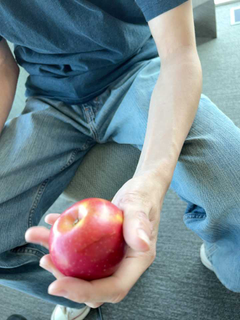
\includegraphics[width=1.30cm,height=1.80cm]{figures/chapters/ch01-basis/cofuse4d-method/assets/input_00118.png}};
    \draw[white,line width=.6pt] (0.95,3.05) rectangle ++(1.30,1.80);
    \draw[cfGray,line width=.35pt,dash pattern=on 1pt off 1pt] (0.55,3.95) -- (0.95,3.10);
    \draw[cfGray,line width=.35pt,dash pattern=on 1pt off 1pt] (0.55,3.95) -- (2.25,3.10);
    \foreach \x/\y/\r in {1.18/3.35/18,1.47/3.75/30,1.75/3.45/22,2.00/3.90/28}{%
      \draw[fill=cfOrange!22,draw=cfOrange,line width=.4pt,rotate around={\r:(\x,\y)}]
        (\x,\y) ellipse (.17 and .065);
    }
    \node[cfTiny,text=cfOrange] at (1.60,2.90) {渲染};
    \node[fill=cfOrange!18,draw=cfOrange,rounded corners=1.2pt,inner sep=1.6pt,
          font=\heiti\fontsize{6.6pt}{8pt}\selectfont,text=cfOrange] at (2.75,4.35) {RGB};
    \node[fill=cfBlue!12,draw=cfBlue,rounded corners=1.2pt,inner sep=1.6pt,
          font=\heiti\fontsize{6.6pt}{8pt}\selectfont,text=cfBlue] at (2.75,3.95) {Depth};
    \node[fill=cfGreen!14,draw=cfGreen,rounded corners=1.2pt,inner sep=1.6pt,
          font=\heiti\fontsize{6.6pt}{8pt}\selectfont,text=cfGreen] at (2.75,3.55) {Track};
    \node[cfTiny,anchor=west,text width=1.75cm] at (2.55,3.10) {光度 / 几何 / 轨迹监督};

    % 3) joint update and outputs
    \draw[fill=white,draw=cfGreen,line width=.7pt,rounded corners=2pt] (0.35,1.45) rectangle (1.75,2.05);
    \node[cfSmall,text=cfGreen] at (1.05,1.75) {GP 运动};
    \draw[fill=white,draw=cfOrange,line width=.7pt,rounded corners=2pt] (2.85,1.45) rectangle (4.25,2.05);
    \node[cfSmall,text=cfOrange] at (3.55,1.75) {高斯表示};
    \draw[cfGray,line width=.8pt,-{Latex[length=1.4mm,width=1mm]}] (1.82,1.88) .. controls (2.15,2.28) .. (2.78,1.88);
    \draw[cfGray,line width=.8pt,-{Latex[length=1.4mm,width=1mm]}] (2.78,1.62) .. controls (2.15,1.22) .. (1.82,1.62);
    \node[cfTiny,text=cfGray] at (2.30,2.18) {联合更新};
    \path[fill=cfOrange,rounded corners=2.2pt] (0.35,0.35) rectangle (4.35,1.18);
    \node[font=\heiti\fontsize{7.6pt}{9pt}\selectfont,text=white] at (2.35,0.90) {PCK@24 77.1 $\to$ 86.5};
    \node[font=\songti\fontsize{6.9pt}{8.2pt}\selectfont,text=white] at (2.35,0.57) {新视角合成 持平};
    \node[cfTiny,text=cfGray] at (2.35,0.18) {输出};
  \end{scope}

  % ================= arrows =================

\end{tikzpicture}
\endgroup
